\chapter{Introduction}
\label{ch:introduction}

\def\figdir{chapters/ch01_introduction/figures}

%\epigraph{\textit{The easiest way to solve a problem is to deny it exists.}}{Isaac Asimov}

%\begin{quote} 
%	\begin{flushright}
%		\textit{The easiest way to solve a problem\\ is to deny it exists.}
%		
%		--- ~ Prof. Isaac Asimov
%	\end{flushright}
%\end{quote}

\section{Motivation}

\lettrine[lines=3,nindent=0em,loversize=0.1]{T}{he} global population is steadily rising and migrating from rural areas to urban areas which has resulted in an ever growing urban population for past two centuries \citep{Oke2017a}. Therefore, the ecology of the urban system has become one of the primary concerns of the society \citep{pachauri2014climate}. Furthermore, the impact of \textit{climate change}, driven by human activity, on the urban society need to be addressed. Strategies need to developed or refined to accommodate the changing climate and provide a mitigation its growing detrimental effect such as urban heat island (UHI). A lack thereof can not only have implication on the global climate but also the comfort and health of urban populace. 

Vegetation, a non-human product, provides natural cooling through shading and transpiration. We see it as a primary and necessary solution to combat the growing UHI and improve the thermal comfort in cities \citep{Gillner2015, Bowler2010, Loughner2012}. Towards this, there is presently a growing need to accurately predict the impact of vegetation at scale of pedestrians. 

The complexifiers which makes urban greening strategies non-trivial is that cooling provided by vegetation is fundamentally environmentally dependent such as the ambient hygrothermal conditions (i.e., air temperature, relative humidity), solar radiation, and the water availability. Figure \ref{fig:vegetation_fluxes} shows a schematic representation of the various fluxes exchanged between an urban tree and the environment. The figure shows that vegetation interacts with multiple coupled physical processes in an urban area. The solar radiation is absorbed by plant foliage and is a main component in the energy balance of the vegetation. The latent (i.e., due to transpiration of moisture) and sensible heat flux from the plant is directly related to the solar radiation intensity. The additional flux of latent heat from vegetation provides the well documented cooling due to transpiration \citep{Oke2017,Farquhar2007, abtew2012evaporation,Melesse2008}. Furthermore, due to the interception of solar radiation by the plant foliage, vegetation provides additional cooling due to shading. Vegetation also has an impact on the water cycle, where the moisture flux at the leaves is dependent on the moisture in the soil. Ergo, the plant transpiration is not only dependent on the ambient atmospheric condition, but also is dependent on the water availability at the plant roots. In other aspect, high vegetation density can also have a negative impact on the ventilation characteristics at the pedestrian level \citep{Gromke2011,Gromke2008}. So, increasing the thermal comfort in urban area could potential be at the cost of air quality. 

\begin{figure}[t]
	\centering
	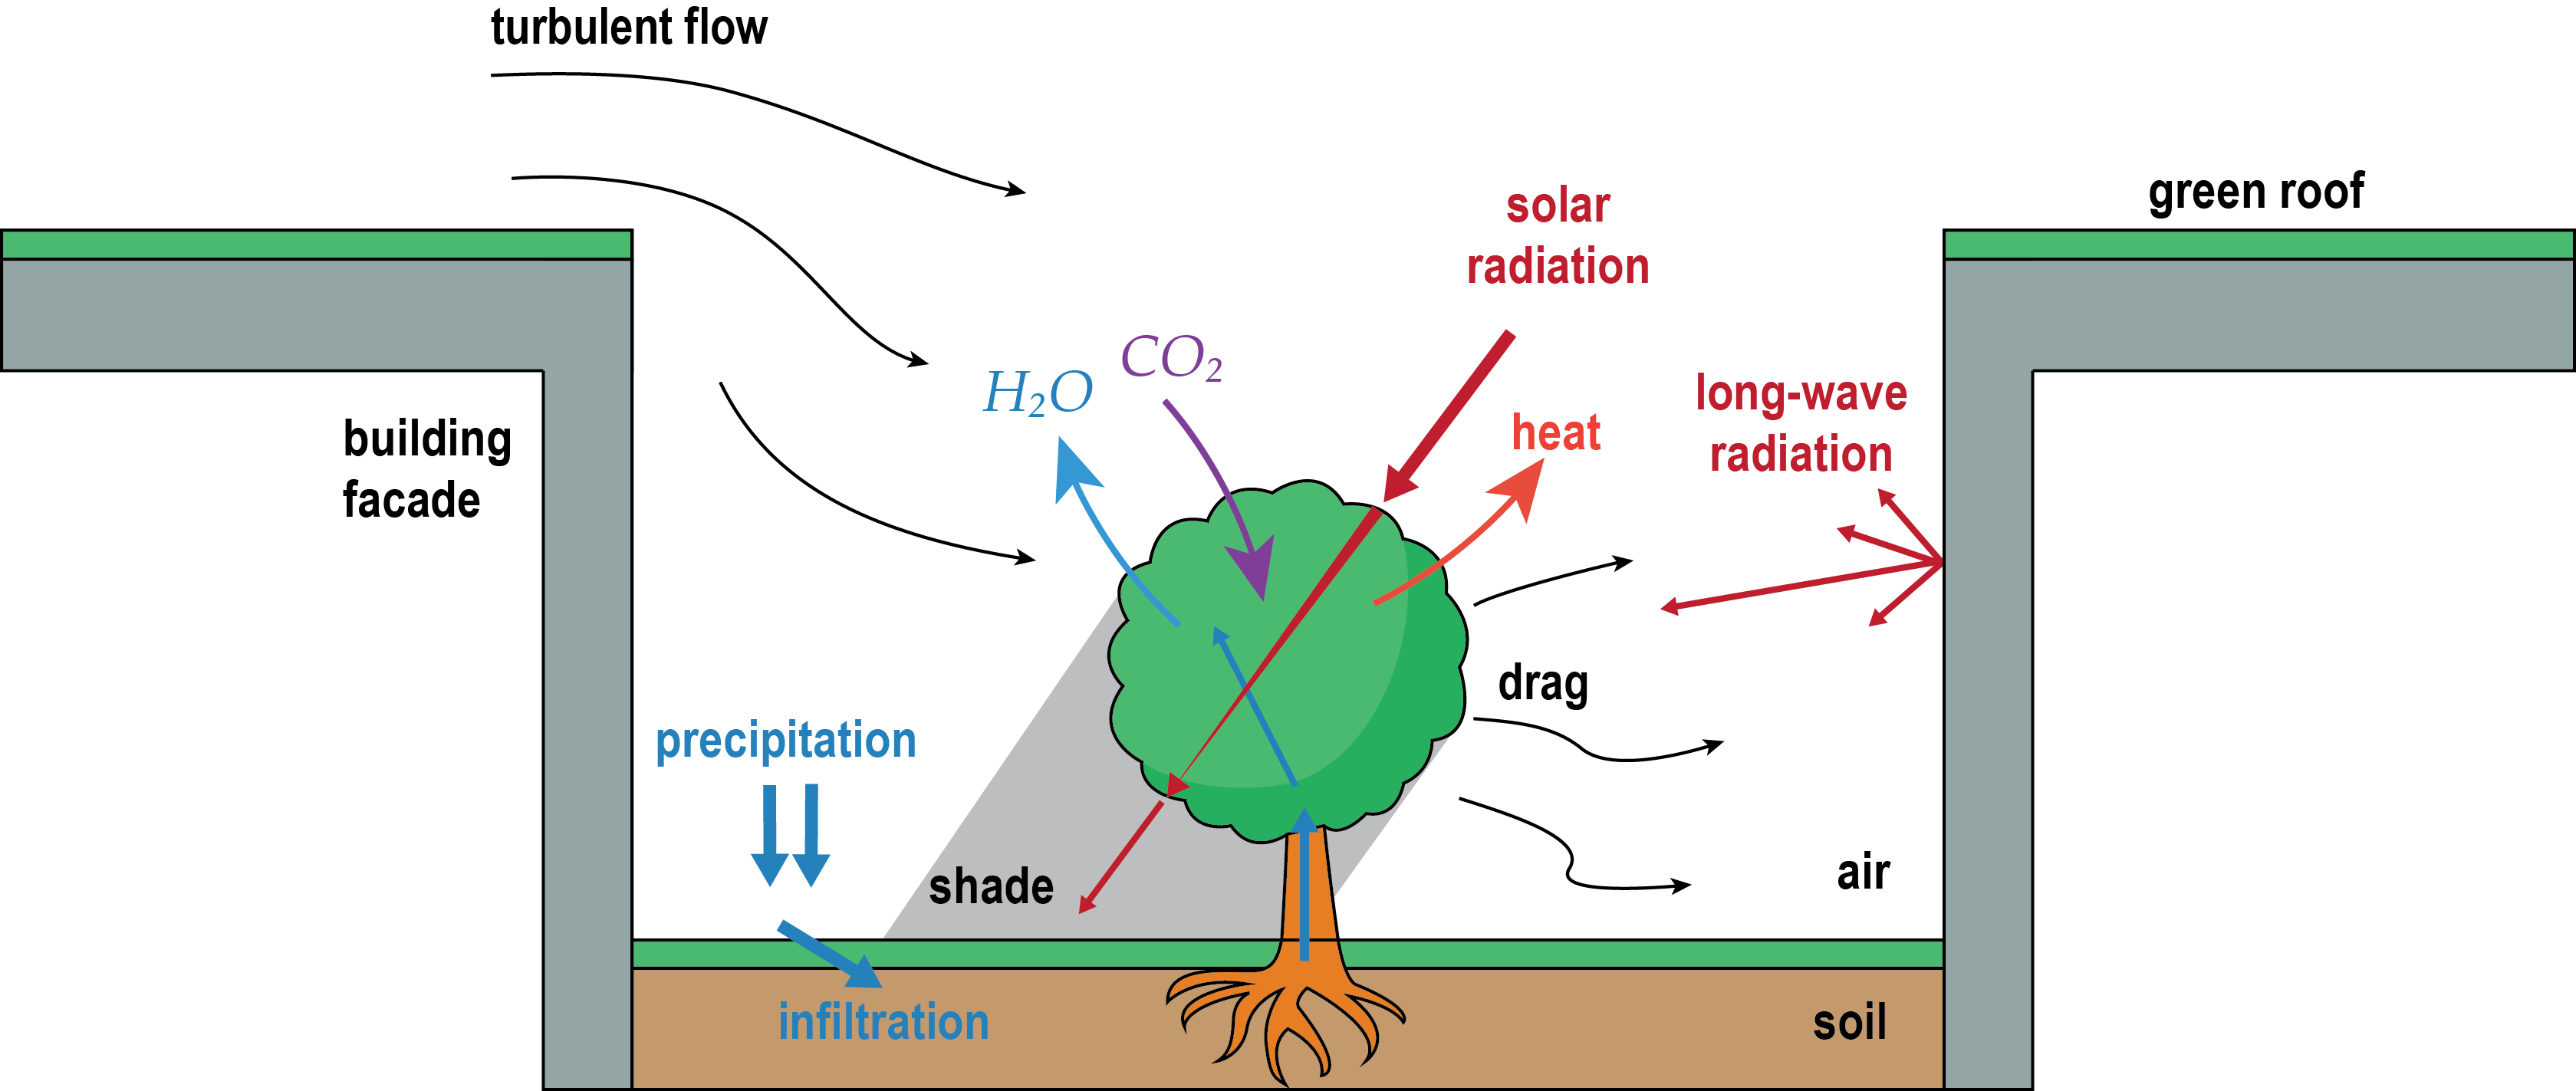
\includegraphics[width=\textwidth]{\figdir/streetcanyon_tree_part5.png}
	\caption{Impact of vegetation on urban microclimate.}
	\label{fig:vegetation_fluxes}
\end{figure}

For this reasons, we can see a need for an multi-domain integrated numerical prediction tool that can take into account of all these factors to provide an accurate assessments on the impact of vegetation in urban microclimate. The numerical method should be able to provide an understanding on the impact of water stress on the transpirative cooling potential of vegetation in cities. It should be able to answer how does the water stress influence the thermal comfort provided by vegetation. Furthermore, experimental research has shown that there is a great need of high-resolution experimental data providing the spatial and temporal variablity in the plant responses to the environment. Specifically, the microclimate around vegetation has been seldom studied in wind tunnels. Wind tunnel experiments are a great tool in experimentally assessing impact of change in urban morphology and the physics of urban flows. Typically, model trees or similar representation are employed to study the impact of vegetation in such urban geometry. Whether small model trees can accurately represent the aerodynamic characteristics of mature trees in cities needs to addressed as well. 

\section{Objective and Methodology}

The goal of the thesis is to improve the assessment on the impact of vegetation on the urban microclimate. As vegetation is increasingly being sought after as a natural UHI mitigation strategy, accurate predictions are need to assess their effectiveness. More specifically, the objective of this thesis is as follows:
\begin{itemize}
	\item to assess the impact of vegetation on the microclimate.
	
	\item to quantify the natural cooling (i.e., transpirative cooling and shading) provided by vegetation in urban microclimate.
	
	\item to understand the influence of water stress on the natural cooling.
	
	\item to quantify the impact of vegetation on pedestrian thermal comfort. 
\end{itemize}

Experimental and numerical approaches are employed to assess the impact of vegetation on the microclimate. Wind tunnel experiments in an atmospheric boundary layer (ABL) are opted to understand the impact of vegetation on the airflow and the local microclimate, where small model trees and small natural trees are employed as scaled models. Measurement techniques such as particle image velocimetry (PIV) and drag force measurement are employed to quantify the modification of airflow due to vegetation. Measurement techniques such as infrared thermography, and hygrothermal sensor analysis are used to quantify the change in hygrothermal variables. A numerical asssessment on the impact of vegetation on urban microclimate is achieved by developing a vegetation model integrated into a computation fluid dynamics  (CFD) model. The numerical model simultaniously takes in account of the turbulence modification, radiation balance, heat and mass fluxes, and the sensitivity to soil moisture simultaneously. With this modeling technique, the cooling potential of vegetation is quantified along with the impact on thermal comfort for a pedestrian. 

Thus, the thesis aims at establishing a more accurate and detailed prediction of the thermal influence of vegetation in an urban environment in OpenFOAM by simultaneously taking in account of its heat, mass, momentum and radiative exchanges. Furthermore, the influence of the water availability on the transpiration rate is modeled using a soil-plant-atmosphere continuum modeling approach. 

\section{Outline of the thesis}

This thesis is divided into two parts: i) experimental studies (\cref{ch:paper2,ch:microclimatestudy}), and ii) numerical studies (\cref{ch:parametricstudy,ch:wtcfdcomparison,ch:numericalmethod,ch:impactofvegetation}) of the impact of vegetation on urban microclimate. The thesis is organized as follow:
\begin{itemize}
	\item \textit{Chapter 2}: The chapter addresses the state of the art providing an overview on the urban climate, the impact of vegetation on urban microclimate, experimental approaches for assessing the impact of vegetation, and numerical approaches for assessing the impact of vegetation in urban microclimate. The goal of the chapter is: i) to provide relevant researches that are present and are employed for determining the impact of vegetation in urban microclimate, ii) to provide a justification on the development of the numerical model that is presented in this thesis, and iii) to give the scope of the numerical model. 

	\item \textit{Chapter 3}: This chapter is the first part of the experimental studies, where the impact of vegetation on the airflow is investigated. The influence of vegetation on the airflow is studied in an atmospheric boundary layer (ABL) wind tunnel using model and small natural trees. In the study, the turbulent airflow behind the trees is studies using particle image velocimetry (PIV) measurement technique and is linked to the drag force measurements using a load cell. The chapter has been published as: Manickathan, L., Defraeye, T., Allegrini, J., Derome, D., \& Carmeliet, J. (2018). ``Comparative study of flow field and drag coefficient of model and small natural trees in a wind tunnel''. \textit{Urban Forestry \& Urban Greening}, 230–239. \url{http://doi.org/10.1016/j.ufug.2018.09.011}.
	%The study investigates the sheltering provided by small model trees and how it differs from that of small natural trees. Thereafter, the flow field and drag coefficient of model trees are compared to the ones of natural trees of similar size to determine whether model trees can be used to represent natural trees. 
	
	\item \textit{Chapter 4}: This chapter is the second part of the experimental studies, where the impact of vegetation on the microclimate is investigated. The influence of vegetation on the microclimate is studied in the wind tunnel using small plant: \textit{Buxus sempervirens}. In the study, the diurnal dynamics of the plant microclimate of a \textit{Buxus sempervirens} is investigated using various high-resolution non-intrusive imaging techniques. The wake flow field is measured using stereoscopic particle image velocimetry (SPIV), the spatiotemporal leaf temperature history is obtained using infrared thermography, and the plant microstructure metrics such as plant porosity, leaf area density (LAD) is obtained through X-ray tomography. %The study helps us answers the following questions: What is the spatial and temporal variability of the plant cooling due to environmental conditions such as wind speed and solar radiation? What is the diurnal response of the plant? Moreover, the experiment provides a high-resolution dataset for future validation studies.
	
	\item \textit{Chapter 5}: This chapter is the first part of the numerical studies, where the impact of vegetation on the transpirative cooling potential is investigated. The influence of vegetation on the transpirative cooling is studied using a computation fluid dynamics (CFD) modeling approach, where vegetation is modeled as porous medium. In the chapter, a parametric study on the influence of environmental factors (i.e., wind speed, air temperature, relative humidity and solar radiation intensity) and tree properties (i.e., leaf size, stomatal resistance and leaf area density) on the transpirative cooling effect of trees is performed. Furthermore, the Universal Thermal Climate Index (UTCI) around the trees is evaluated to determine the impact of transpirative cooling on pedestrian thermal comfort. The chapter has been published as: Manickathan, L., Defraeye, T., Allegrini, J., Derome, D., \& Carmeliet, J. (2018). ``Parametric study of the influence of environmental factors and tree properties on the transpirative cooling effect of trees''. \textit{Agricultural and Forest Meteorology}, 248, 259–274. \url{http://doi.org/10.1016/j.agrformet.2017.10.014}.%It porous medium approach provides the necessary source terms for heat, mass, momentum, and radiative fluxes due to vegetation. 
	
	\item \textit{Chapter 6}: This chapter is focuses on comparing the developed numerical in \cref{ch:parametricstudy} with wind tunnel measurements of \cref{ch:microclimatestudy}. The goal of the chapter is to compare and determine the discrepancy of the numerical model in predicting the airflow and the transpiration cooling of vegetation. 
	
	\item \textit{Chapter 7}: This chapter the numerical model of assessing the impact of vegetation in urban microclimate is described. The \textit{air} domain solver, the \textit{solid} domain solver, and the \textit{radiation} model is described in detail. Furthermore, the chapter describes the coupling strategy employed to couple these three models which an overview of the coupling algorithm. The influence of water availability on transpiration rate is addressed using a modified stomatal model based on the soil-plant-atmosphere continuum (SPAC) model approach. 
	
	\item \textit{Chapter 8}: This chapter is the second part of the numerical studies, where the impact of vegetation on the urban microclimate is investigated using the numerical model described in \cref{ch:numericalmethod}. The impact of vegetation on the urban microclimate consists of modification to the urban turbulent airflow, addition of transpirative cooling in urban area, and the plant shading provided by the foliage. The influence of these phenomena is investigated together with the impact of pedestrian thermal comfort. 
	
	\item \textit{Chapter 9}: Finally, this chapter provides a conclusion and some of the main finding in the thesis. Furthermore, the chapter provides an overview to the contributions to the research field from the present thesis. An outlook and possible future research aspects is given thereafter.
	
\end{itemize}

